\section{Data Description Frameworks}
\label{sec: data-formats}


Many application developers rely on data description frameworks or libraries to manage data types\footnote{A datatype is a collection of properties, all of which can be stored on storage and which, when taken as a whole, provide complete information for data conversion to or from the datatype.}.
Different libraries and middleware provide mechanisms to describe data using basic types and to construct new ones using dedicated APIs.
Data types are provided as a transparent conversion mechanism between internal representation (as data is represented in memory) and external representation (how data is transmitted over the network or saved to permanent storage).
This section gives an overview of data types provided by different software packages.
Starting from existing middleware and datatype definitions, we will propose a list of basic data types to be supported by the ESD middleware.

%The benefits are manifold and many different projects are available.

%%%%%%%%%%%%%%%%%%%%%%%%%%%%%%%%%%%%%%%%%%%%%%%%%%%%%%%%%%%%%%%%%%%%%%%%%%%%%%%
\subsection{MPI}
The Message Passing Interface supports derived data types for efficient data transfer as well as a short description of file layouts (through file views). MPI defines a set of basic data types (or type class) from which more complex ones can be derived using appropriate data constructor APIs. Basic datatypes in MPI resemble C atomic types as shown in \Cref{table: mpi-types}.

\clearpage

\begin{longtable}{|>{\centering\arraybackslash} m{5.5cm} | >{\centering\arraybackslash} m{6cm} |}\hline\hline
        \cellHeader Datatype                  & \cellHeader Description                                                               \\ \hline
        \small \texttt{MPI\_CHAR}                     & \small this is the traditional ASCII character that is numbered by integers between 0 and 127 \\ \hline
        \small \texttt{MPI\_WCHAR}                    & \small this is a wide character, e.g., a 16-bit character such as a Chinese ideogram          \\ \hline
        \small \texttt{MPI\_SHORT}                    & \small this is a 16-bit integer between -32,768 and 32,767                                    \\ \hline
        \small \texttt{MPI\_INT}                      & \small this is a 32-bit integer between -2,147,483,648 and 2,147,483,647                      \\ \hline
        \small \texttt{MPI\_LONG}                     & \small this is the same as MPI\_INT on IA32                                                   \\ \hline
        \small \texttt{MPI\_LONG\_LONG\_INT}          & \small this is a 64-bit long signed integer, i.e., %
                                                        an integer number between -9,223,372,036,854,775,808 and 9,223,372,036,854,775,807            \\ \hline
        \small \texttt{MPI\_LONG\_LONG}               & \small same as MPI\_LONG\_LONG\_INT                                                           \\ \hline
        \small \texttt{MPI\_SIGNED\_CHAR}             & \small same as MPI\_CHAR                                                                      \\ \hline
        \small \texttt{MPI\_UNSIGNED\_CHAR}           & \small this is the extended character numbered by integers between 0 and 255                  \\ \hline
        \small \texttt{MPI\_UNSIGNED\_SHORT}          & \small this is a 16-bit positive integer between 0 and 65,535                                 \\ \hline
        \small \texttt{MPI\_UNSIGNED\_LONG}           & \small this is the same as MPI\_UNSIGNED on IA32                                              \\ \hline
        \small \texttt{MPI\_UNSIGNED}                 & \small this is a 32-bit unsigned integer, i.e., a number between 0 and 4,294,967,295          \\ \hline
        \small \texttt{MPI\_FLOAT}                    & \small this is a single precision, 32-bit long floating point number                          \\ \hline
        \small \texttt{MPI\_DOUBLE}                   & \small this is a double precision, 64-bit long floating point number                          \\ \hline
        \small \texttt{MPI\_LONG\_DOUBLE}             & \small this is a quadruple precision, 128-bit long floating point number                      \\ \hline
        \small \texttt{MPI\_C\_COMPLEX}               & \small this is a complex float                                                                \\ \hline
        \small \texttt{MPI\_C\_FLOAT\_COMPLEX}        & \small same as MPI\_C\_COMPLEX                                                                \\ \hline
        \small \texttt{MPI\_C\_DOUBLE\_COMPLEX}       & \small this is a complex double                                                               \\ \hline
        \small \texttt{MPI\_C\_LONG\_DOUBLE\_COMPLEX} & \small this is a long double complex                                                          \\ \hline
        \small \texttt{MPI\_C\_BOOL}                  & \small this is a \_Bool                                                                       \\ \hline
        \small \texttt{MPI\_INT8\_T}                  & \small this is a 8-bit integer                                                                \\ \hline
        \small \texttt{MPI\_INT16\_T}                 & \small this is a 16-bit integer                                                               \\ \hline
        \small \texttt{MPI\_INT32\_T}                 & \small this is a 32-bit integer                                                               \\ \hline
        \small \texttt{MPI\_INT64\_T}                 & \small this is a 64-bit integer                                                               \\ \hline
        \small \texttt{MPI\_UINT8\_T}                 & \small this is a 8-bit unsigned integer                                                       \\ \hline
        \small \texttt{MPI\_UINT16\_T}                & \small this is a 16-bit unsigned integer                                                      \\ \hline
        \small \texttt{MPI\_UINT32\_T}                & \small this is a 32-bit unsigned integer                                                      \\ \hline
        \small \texttt{MPI\_UINT64\_T}                & \small this is a 64-bit unsigned integer                                                      \\ \hline
        \small \texttt{MPI\_BYTE}                     & \small this is an 8-bit positive integer                                                      \\ \hline
        \small \texttt{MPI\_PACKED}                   & -                                                                                             \\ \hline
        \caption{MPI Datatypes}
        \label{table: mpi-types}
\end{longtable}

Data types from Table~\ref{table: mpi-types} can be used in combination with the constructor APIs shown in Table~\ref{table: mpi-constr} to build more complex derived data types.

\begin{longtable}{|>{\centering\arraybackslash} m{5.5cm} | >{\centering\arraybackslash} m{6cm} |}\hline\hline
        \cellHeader Datatype Constructor           & \cellHeader Description                               \\ \hline
        \small \texttt{MPI\_Type\_create\_hindexed}        & \small create an indexed datatype with displacement in bytes  \\ \hline
        \small \texttt{MPI\_Type\_create\_hindexed\_block} & \small create an hindexed datatype with constant-sized blocks \\ \hline
        \small \texttt{MPI\_Type\_create\_indexed\_block}  & \small create an indexed datatype with constant-sized blocks  \\ \hline
        \small \texttt{MPI\_Type\_create\_keyval}          & \small create an attribute keyval for MPI data types           \\ \hline
        \small \texttt{MPI\_Type\_create\_hvector}         & \small create a datatype with constant stride given in bytes  \\ \hline
        \small \texttt{MPI\_Type\_create\_struct}          & \small create a MPI datatype from a general set of data types, %
                                                             displacements and block sizes                                 \\ \hline
        \small \texttt{MPI\_Type\_create\_darray}          & \small create a datatype representing a distributed array     \\ \hline
        \small \texttt{MPI\_Type\_create\_resized}         & \small create a datatype with a new lower bound and extent %
                                                             from an existing datatype                                     \\ \hline
        \small \texttt{MPI\_Type\_create\_subarray}        & \small create a datatype for a subarray of a regular, %
                                                             multidimensional array                                        \\ \hline
        \small \texttt{MPI\_Type\_contiguous}              & \small create a contiguous datatype                           \\ \hline
        \caption{MPI Derived Datatypes Constructors}
        \label{table: mpi-constr}
\end{longtable}

Before they can be used, MPI derived data types (created using the constructors in Table~\ref{table: mpi-constr}) have to be committed to memory using the \texttt{MPI\_Type\_commit} interface.
Similarly, when no longer needed, derived data types can be freed using the \texttt{MPI\_Type\_free} interface.
Unlike data format libraries, MPI does not provide any permanent data representation (MPI-IO can only read/write binary data), therefore derived data types are not used to store any specific data format on stable storage and are instead used only for data transfers or file layout descriptions.

Example code for defining a derived data structure for a structure is shown in \Cref{lst:mpi-struct}.
The structure is defined in Lines 5-9.
The function in Lines 12-22 registers this datatype in MPI.
It is required to define the beginning and end of each array, its type and size.
Once a datatype is defined, it can be used as memory type in subsequent operations.
In this example, one process sends this datatype to another process (Line 38 and Line 45).

Since MPI data types were initially designed for computation and, thus, to define memory regions, they do not offer a way to name the data structures.

\begin{tcbcode}[label={lst:mpi-struct}]{Example construction of an MPI datatype for a structure}
\begin{lstlisting}[language=c++,morekeywords={{student_t}}]
#include <stdio.h>
#include <string.h>
#include <mpi.h>

typedef struct student_t_s {
    int id[2];
    float grade[5];
    char name[20];
} student_t;

/* create a type for the struct student_t */
void create_student_datatype(MPI_Datatype * mpi_student_type){
    int   blocklengths[3] = {2, 5, 20};
    MPI_Datatype types[3] = {MPI_INT, MPI_FLOAT, MPI_CHAR};
    MPI_Aint     offsets[3];

    offsets[0] = offsetof(student_t, id) ;
    offsets[1] = offsetof(student_t, grade);
    offsets[2] = offsetof(student_t, name);
    MPI_Type_create_struct(3, blocklengths, offsets, types, mpi_student_type);
    MPI_Type_commit(mpi_student_type);
}

int main(int argc, char **argv) {
    const int tag = 4711;
    int size, rank;

    MPI_Init(&argc, &argv);
    MPI_Comm_size(MPI_COMM_WORLD, &size);
    MPI_Comm_rank(MPI_COMM_WORLD, &rank);

    MPI_Datatype mpi_student_type;
    create_student_datatype(& mpi_student_type);

    if (rank == 0) {
        student_t send = {{1, 2},  {1.0, 2.0, 1.7, 2.0, 1.7},  "Nina Musterfrau"};
        const int target_rank = 1;
        MPI_Send(&send,   1, mpi_student_type, target_rank, tag, MPI_COMM_WORLD);
    }
    if (rank == 1) {
        MPI_Status status;
        const int src=0;
        student_t recv;
        memset(& recv, 0, sizeof(student_t));
        MPI_Recv(&recv,   1, mpi_student_type, src, tag, MPI_COMM_WORLD, &status);
        printf("Rank %d: Received: id = %d grade = %f student = %s\n", rank, recv.id[0], recv.grade[0], recv.name);
    }

    MPI_Type_free(&mpi_student_type);
    MPI_Finalize();

    return 0;
}
\end{lstlisting}
\end{tcbcode}



%%%%%%%%%%%%%%%%%%%%%%%%%%%%%%%%%%%%%%%%%%%%%%%%%%%%%%%%%%%%%%%%%%%%%%%%%%%%%%%
\subsection{HDF5}

%The hierarchical data format is...

%\begin{quotation}
%\itshape
HDF5 is a data model, library, and file format for storing and managing data. It supports an unlimited variety of data types and is designed for flexible and efficient I/O and high volume and complex data.
HDF5 is portable and is extensible, allowing applications to evolve in their use of HDF5.
The HDF5 Technology suite includes tools and applications for managing, manipulating, viewing, and analysing data in the HDF5 format. Like MPI, HDF5 also supports its own basic (native) data types reported in \Cref{table: hdf5-types}.
%\end{quotation}

\begin{longtable}{|>{\centering\arraybackslash} m{5.5cm} | >{\centering\arraybackslash} m{6cm} |}\hline\hline
        \cellHeader Datatype        & \cellHeader Corresponding C Type                  \\ \hline
        \small \texttt{H5\_NATIVE\_CHAR}    & \small \texttt{char}                                      \\ \hline
        \small \texttt{H5\_NATIVE\_SCHAR}   & \small \texttt{signed char}                               \\ \hline
        \small \texttt{H5\_NATIVE\_UCHAR}   & \small \texttt{unsigned char}                             \\ \hline
        \small \texttt{H5\_NATIVE\_SHORT}   & \small \texttt{short}                                     \\ \hline
        \small \texttt{H5\_NATIVE\_USHORT}  & \small \texttt{unsigned short}                            \\ \hline
        \small \texttt{H5\_NATIVE\_INT}     & \small \texttt{int}                                       \\ \hline
        \small \texttt{H5\_NATIVE\_UINT}    & \small \texttt{unsigned int}                              \\ \hline
        \small \texttt{H5\_NATIVE\_LONG}    & \small \texttt{long}                                      \\ \hline
        \small \texttt{H5\_NATIVE\_ULONG}   & \small \texttt{unsigned long}                             \\ \hline
        \small \texttt{H5\_NATIVE\_LLONG}   & \small \texttt{long long}                                 \\ \hline
        \small \texttt{H5\_NATIVE\_ULLONG}  & \small \texttt{unsigned long long}                        \\ \hline
        \small \texttt{H5\_NATIVE\_FLOAT}   & \small \texttt{float}                                     \\ \hline
        \small \texttt{H5\_NATIVE\_DOUBLE}  & \small \texttt{double}                                    \\ \hline
        \small \texttt{H5\_NATIVE\_LDOUBLE} & \small \texttt{long double}                               \\ \hline
        \small \texttt{H5\_NATIVE\_B8}      & \small 8-bit unsigned integer or 8-bit buffer in memory   \\ \hline
        \small \texttt{H5\_NATIVE\_B16}     & \small 16-bit unsigned integer or 16-bit buffer in memory \\ \hline
        \small \texttt{H5\_NATIVE\_B32}     & \small 32-bit unsigned integer or 32-bit buffer in memory \\ \hline
        \small \texttt{H5\_NATIVE\_B64}     & \small 64-bit unsigned integer or 64-bit buffer in memory \\ \hline
        %\small \texttt{H5\_NATIVE\_OPAQUE} & \small \\ \hline
        \small \texttt{H5\_NATIVE\_HADDR}   & \small \texttt{haddr\_t}                                  \\ \hline
        \small \texttt{H5\_NATIVE\_HSIZE}   & \small \texttt{hsize\_t}                                  \\ \hline
        \small \texttt{H5\_NATIVE\_HSSIZE}  & \small \texttt{hssize\_t}                                 \\ \hline
        \small \texttt{H5\_NATIVE\_HERR}    & \small \texttt{herr\_t}                                   \\ \hline
        \small \texttt{H5\_NATIVE\_HBOOL}   & \small \texttt{hbool\_t}                                  \\ \hline
        \caption{HDF5 Native Datatypes}
        \label{table: hdf5-types}
\end{longtable}

Besides the native data types, the library also provides so-called standard data types, architecture specific data types (e.g., for i386), IEEE floating point data types, and others.
Data types can be built or modified starting from the native set of data types using the constructors as listed in \Cref{table: hdf5-constr}.

HDF5 constructs allow the user a fine-grained definition of arbitrary data types.
Indeed, HDF5 allows the user to build a user-defined datatype starting from a native datatype (by copying the native type) and then change datatype characteristics like the sign, precision, etc., using the supported datatype constructor API.
However, since these user-defined data types often have no direct representation of available hardware, this can lead to performance issues.

\clearpage

\begin{longtable}{|>{\centering\arraybackslash} m{5.5cm} | >{\centering\arraybackslash} m{6cm} |}\hline\hline
        \cellHeader Datatype Constructor & \cellHeader Description \\ \hline
        \small \texttt{H5Tcreate}                & \small Creates a new datatype of the specified class with the specified number of bytes. This function is used only with the following datatype classes: %
                                                   H5T\_COMPOUND, H5T\_OPAQUE, H5T\_ENUM, H5T\_STRING. %
                                                   Other data types, including integer and floating-point data types, are %
                                                   typically created by using H5Tcopy to copy and modify %
                                                   a predefined datatype                                                               \\ \hline
        \small \texttt{H5Tvlen\_create}          & \small Creates a new one-dimensional array datatype of variable-length (VL) with %
                                                   the base datatype. The base type specified for the VL datatype can be any HDF5 %
                                                   datatype, including another VL datatype, a compound datatype, or an atomic datatype \\ \hline
        \small \texttt{H5Tarray\_create}         & \small Creates a new multidimensional array datatype object                         \\ \hline
        \small \texttt{H5Tenum\_create}          & \small Creates a new enumeration datatype based on the specified base datatype, %
                                                   dtype\_id, which must be an integer datatype                                        \\ \hline
        \small \texttt{H5Tcopy}                  & \small Copies an existing datatype. The returned type is always transient and unlocked. A native datatype can be copied and modified using other APIs %
                                                   (e.g. changing the precision)                                                       \\ \hline
        \small \texttt{H5Tset\_precision}        & \small Sets the precision of an atomic datatype. The precision is the number of significant bits                                                                    \\ \hline
        \small \texttt{H5Tset\_sign}             & \small Sets the sign property for an integer type. The sign can be unsigned or two's complement                                                                    \\ \hline
        \small \texttt{H5Tset\_size}             & \small Sets the total size in bytes for a datatype                                  \\ \hline
        \small \texttt{H5Tset\_order}            & \small Sets the byte order of a datatype (big endian or little endian)              \\ \hline
        \small \texttt{H5Tset\_offset}           & \small Sets the bit offset of the first significant bit                             \\ \hline
        \small \texttt{H5Tset\_fields}           & \small Sets the locations and sizes of the various floating-point bit fields. The field positions are bit positions in the significant region of the datatype. Bits are numbered with the least significant bit number zero                        \\ \hline
        \caption{HDF5 Data types Constructors}
        \label{table: hdf5-constr}
\end{longtable}

\clearpage

%%%%%%%%%%%%%%%%%%%%%%%%%%%%%%%%%%%%%%%%%%%%%%%%%%%%%%%%%%%%%%%%%%%%%%%%%%%%%%%
\subsection{NetCDF}

NetCDF is a crucial and popular alternative within the climate community. NetCDF provides a set of software libraries and self-describing, machine-independent, data formats that support the creation, access, and sharing of array-oriented scientific data.
In version 4 of the library (NetCDF4), the used binary file representation is HDF5. Like MPI and HDF5, NetCDF also defines its own set of atomic data types as shown in \Cref{table: netcdf-types}.
%\end{quotation}

\begin{table}
\centering
\begin{tabular}{|>{\centering\arraybackslash} m{5.5cm} | >{\centering\arraybackslash} m{6cm} |}\hline\hline
        \cellHeader Datatype & \cellHeader Description         \\ \hline
        \small \texttt{NC\_BYTE}     & \small 8-bit signed integer             \\ \hline
        \small \texttt{NC\_UBYTE}    & \small 8-bit unsigned integer           \\ \hline
        \small \texttt{NC\_CHAR}     & \small 8-bit character byte             \\ \hline
        \small \texttt{NC\_SHORT}    & \small 16-bit signed integer            \\ \hline
        \small \texttt{NC\_USHORT}   & \small 16-bit unsigned integer          \\ \hline
        \small \texttt{NC\_INT}      & \small 32-bit signed integer            \\ \hline
        \small \texttt{NC\_UINT}     & \small 32-bit unsigned integer          \\ \hline
        \small \texttt{NC\_INT64}    & \small 64-bit signed integer            \\ \hline
        \small \texttt{NC\_UINT64}   & \small 64-bit unsigned integer          \\ \hline
        \small \texttt{NC\_FLOAT}    & \small 32-bit floating point            \\ \hline
        \small \texttt{NC\_DOUBLE}   & \small 64-bit floating point            \\ \hline
        \small \texttt{NC\_STRING}   & \small variable length character string \\ \hline
\end{tabular}
        \caption{netCDF Atomic External Datatypes}
        \label{table: netcdf-types}
\end{table}


Similarly, to HDF5 and MPI, in addition to the atomic types, the user can define their own types. NetCDF supports four different user-defined types:
%
\begin{enumerate}
        \item \textbf{Compound}: are a collection of types (either user defined or atomic)
        \item \textbf{Variable Length Arrays}: are used to store non-uniform arrays
        \item \textbf{Opaque}: only contain the size of each element and no datatype information
        \item \textbf{Enum}: like an enumeration in C
\end{enumerate}

Once types are constructed, variables of the new type can be instantiated with \texttt{nc\_def\_var}. Data can be written to the new variable using  \texttt{nc\_put\_var1}, \texttt{nc\_put\_var}, \texttt{nc\_put\_vara}, or \texttt{nc\_put\_vars}. Data can be read from the new variable with \texttt{nc\_get\_var1}, \texttt{nc\_get\_var}, \texttt{nc\_get\_vara}, or \texttt{nc\_get\_vars}.
Finally, new attributes can be added to the variable using nc\_put\_att, and existing attributes can be accessed from the variable using \texttt{nc\_get\_att}.


\medskip

Table~\ref{table: netcdf-constr} shows the constructors provided to build user-defined data types.

\begin{longtable}{|>{\centering\arraybackslash} m{1.7cm} | >{\centering\arraybackslash} m{4.5cm} | >{\centering\arraybackslash} m{5cm} |}\hline\hline
        \cellHeader Type & \cellHeader Constructor & \cellHeader Description \\ \hline
        \multirow{4}{1.7cm}{\centering \small Compound} %
                                             & \small \texttt{nc\_def\_compound}              & \small create a compound datatype                     \\ \cline{2-3}
                                             & \small \texttt{nc\_insert\_compound}           & \small insert a name field into a compound datatype   \\ \cline{2-3}
                                             & \small \texttt{nc\_insert\_array\_compound}    & \small insert an array field into a compound datatype \\ \cline{2-3}
                                             & \small \texttt{nc\_inq\_\{compound,name,...\}} & \small learn information about a compound datatype    \\ \hline
        \multirow{3}{1.7cm}{\centering \small Variable Length Array}%
                                             & \small \texttt{nc\_def\_vlen}                  & \small create a variable length array                 \\ \cline{2-3}
                                             & \small \texttt{nc\_inq\_vlen}                  & \small learn about a variable length array            \\ \cline{2-3}
                                             & \small \texttt{nc\_free\_vlen}                 & \small release memory from a variable length array    \\ \hline
        \multirow{2}{1.7cm}{\centering \small Opaque} %
                                             & \small \texttt{nc\_def\_opaque}                & \small create an opaque datatype                      \\ \cline{2-3}
                                             & \small \texttt{nc\_inq\_opaque}                & \small learn about an opaque datatype                 \\ \hline
        \multirow{3}{1.7cm}{\centering \small Enum} %
                                             & \small \texttt{nc\_def\_enum}                  & \small create an enum datatype                        \\ \cline{2-3}
                                             & \small \texttt{nc\_insert\_enum}               & \small insert a named member into an enum datatype    \\ \cline{2-3}
                                             & \small \texttt{nc\_inq\_\{enum,...\}}          & \small learn information about an enum datatype       \\ \hline
        \caption{NetCDF Datatypes Constructors}
        \label{table: netcdf-constr}
\end{longtable}
\newpage




%%%%%%%%%%%%%%%%%%%%%%%%%%%%%%%%%%%%%%%%%%%%%%%%%%%%%%%%%%%%%%%%%%%%%%%%%%%%%%%
\subsection{GRIB}
%unlike HDF5, NetCDF or MPI grib specifies messages which can contain certain data sections

%GRIB is widely used
%and standardised by \cite{WMO}
GRIB is a library and data format commonly used in weather applications.
It differs from previously described libraries in the sense that it does not define datatypes that can be used to store a wide range of different data.
Instead, GRIB very clearly defines the sections of every -- so-called -- message which is the unit sent across a network link or written to permanent storage.
Every message in GRIB has different sections, each of which contains some information.
GRIB defines the units that can be represented in every message and thus does not explicitly need datatypes to represent them.
But a library supporting these formats needs to know the mapping from a message type to the contained data fields and their data types.
In that sense, GRIB is not a self-describing file format but requires a code to define the standardised content.
GRIB messages contain 32-bit integers that can be scaled using a predefined data packing schema. The scaling factor is stored along with the data inside the message.


%%%%%%%%%%%%%%%%%%%%%%%%%%%%%%%%%%%%%%%%%%%%%%%%%%%%%%%%%%%%%%%%%%%%%%%%%%%%%%%
\section{Storage Systems}
\label{sec: background/storage systems}

This section introduces interesting storage systems, in particular, software concepts.
With ESD, we focus on HPC. However, other fields are very active in the creation of storage systems with embedded processing engines.
Since we use some low-level concepts which are exploited by existing software products, we introduce these solutions briefly.
ESD directly uses some of the listed systems.

\subsection{WOS}
\label{WOS background}

DDN (Data Direct Network) WOS (Web object scaler)\footnote{\url{http://www.ddn.com/products/object-storage-web-object-scaler-wos/}} represents an object storage solution able to manage files as ``objects''.

It offers a simple and effective way to manage data stored in the cloud through an ease administration interface and IP based direct connection to the nodes.
WOS architecture is natively geographically agnostic, and this represents one of the main features of the product: nodes can be deployed anywhere, and the access to data which they host is guaranteed by Internet Protocol (IP) connectivity.
In this sense, all the nodes which form the cloud work together to create an aggregated pool of storage space.

WOS relies on the following features and concepts:
\begin{itemize}
\item \textbf{nodes, zones and cloud}: nodes represent the addressable elements of the architecture; they participate in the cloud environment providing their storage space and computational power.
The nodes are connected to the WOS cloud through a preferably high-speed internet connection.
Multiple nodes form a zone which collects nodes with a specific policy. The WOS system is able to balance the load among the nodes within a zone automatically.
The pool of the zones forms the entire WOS cloud, and the membership of a common network guarantees the communication in the cloud.
\item \textbf{policy}: the administrator defines different rules which determine the object distribution. It is important to highlight that files + metadata + policy form an Object.
\item \textbf{object:} an object is formed by multiple elements managed by WOS as a single entity. For instance, an object could be a file stored in the WOS cloud or a group of them.
\item \textbf{Object ID (OID)}: An OID uniquely identifies an object (and its replicas, if any). The OID has to be provided to the WOS system for allowing the addressing and retrieving of the related object.
\end{itemize}
In addition to these, WOS supports the definition of metadata by the users in the form of key-value pairs and multiple replicas for each object (managed by the policy rules).

WOS cloud is an excellent solution to take into account to manage data in environments which present particular features or challenges that could affect the traditional architectures based on common file-systems and storage solutions.
For example, this cloud can be successfully applied when data sets are too large for a single file system and, so, they need to be stored on multiple sites or, on the contrary, there are large quantities of files which are very small.
Other examples are systems that present high rates of file read, write and/or file deletion or if users want a small system to start with the possibility to easily scale up.
The only requirements of a WOS installation are related to the connection between the nodes: nodes must be interconnected through a network (LAN or WAN or a combination of them) and must be able to communicate using the TCP/IP protocol.
The network between the nodes should be stable and reliable (anyway WOS system are able to recover the regular operational activity after a network outages), fast (multiple Gigabit ports are preferred or 10 Gigabit Ethernet connections) and low-latency (which is an important aspect especially for TCP/IP connections so using low-latency appliances will guarantee the best results).

The WOS Core relies on three main services and an instance of each service is installed on each node that forms the WOS cluster. These services are:
\begin{itemize}
\item The\textbf{Management Tuning Service (MTS)} which has the task to control the administration and configuration functions.
The master node hosts the primary MTS while the other nodes host an instance of this service.

\item The \textbf{wosnode} which is hosted on each node of the cluster. It manages and controls all the I/O operations to the connected devices. The WOS node operates only on the local node also in the case the MTS goes down to improve performance and reliability.

\item The \textbf{wosrest} represents the service which provides the REST (Representational State Transfer) interface. An application that accesses the WOS cluster over the network interact with the node through this service and the REST interface.
\end{itemize}

\textbf{The WOS API}

WOS architecture provides several APIs for connecting an application to the cluster, manages the objects and the related metadata.
Specifically, WOS provides API for C++, JAVA and Python languages.
In addition, it provides an HTTP Restful interface.
It is not allowed to modified objects so each object can be written only once, read many times and eventually deleted.

As mentioned above, each object has a unique Object-ID (OID) that is returned to the user when the object is created.
OID is unique for the entire life of the cluster, and no OID replication is also allowed if an object is deleted.
OID should be used by the clients to access the object. Therefore, typical applications have to maintain a catalogue for collecting the OID of the stored objects.
In this context, we will analyse the C++ APIs provided by the WOS installation, and the extensions developed to wrap the C++ APIs on C functions.
The C++ APIs provide an interface for the following operations:
\begin{itemize}
	\item Connect to the WOS cluster;
	\item Create WOS objects;
	\item PUT, GET, DELETE, EXISTS (on objects)
	\item Reserve, PutOID (on Object-IDs)
\end{itemize}

Moreover, it offers functionality for supporting streaming features, which allows them to read and write large objects without storing the entire set of data in the client memory and to retrieve metadata independently of the related data.

The following list details the calls for each operation mentioned before.

\begin{longtable}{|>{\centering\arraybackslash} m{3cm} | >{\centering\arraybackslash} m{5cm} | >{\centering\arraybackslash} m{5cm} |}\hline\hline\hline
        \cellHeader Operation & \cellHeader WOS  Call &  \cellHeader Description \\ \hline
	Connect  & \textit{WosClusterPtr wos = WosCluster::Connect(host);} & \textit{host} represents the IP address of one host of the WOS cluster. A process can open only one connection to the cluster and should keep it open until the termination. \\ \hline
	Create object & \textit{WosObjPtr wobj = WosObj::Create();} & \textit{wobj} is a C++ WosObject. After creating a WosObject, data and metadata can be associated \\ \hline
	Set data\newline Set metadata & \textit{wobj-\textgreater SetData(data, len);}\newline \textit{wobj-\textgreater SetMeta("\textless key\textgreater", "value");} & \textit{wobj} represents the WosObject and \textit{data} the void pointer containing the data to store. For metadata, the couple \textit{\textless key\textgreater, \textless value\textgreater} must be passed. \\ \hline
	Put blocking\newline Put non-blocking & \textit{wos-\textgreater Put(status, oid, policy, wobj);}\newline \textit{wos-\textgreater Put(wobj, policy, callback, context);} & \textit{wobj} is the just created WOS Object to put. The non-blocking form needs a \textit{callback} function and a \textit{context} object to perform and synchronise the starting and the termination of the operation. \\ \hline
	Get blocking\newline Get non-blocking & \textit{wos-\textgreater Get(status, oid, wobj);}\newline \textit{wos-\textgreater Get(oid, callback, context);} & as for the put function, the non-blocking case uses a \textit{context} and a \textit{callback} function. After retrieving a WOS object data and metadata included can be read. \\ \hline
	Get data\newline Get metadata & \textit{wobj-\textgreater GetData(data, length);}\newline \textit{wobj-\textgreater GetMeta("\textless key\textgreater", value);} & \textit{wobj} represents the WosObject and \textit{data} the void pointer for storing the retrieved data. To retrieve metadata the corresponding \textit{key} must be passed. It is worth noting that WOS does not allow to modify/update objects: a modified copy could be stored as a separate object \\ \hline
	Delete blocking\newline Delete non-blocking & \textit{wos-\textgreater Delete(status, oid);} \newline \textit{wos- \textgreater Delete(oid, callback, context);} & as for the put and get functions, the \textit{delete} operation can be performed in a blocking or non-blocking form \\ \hline
	Exists blocking\newline Exists non-blocking & wos-\textgreater Exists(status, oid);\newline wos-\textgreater Exists(oid, callback, context);\newline & Check the existence of a WOS Object using its OID. To actually retrieve the object and data the related get functions could be used \\ \hline
	Reserve blocking\newline Reserve non-blocking & wos-\textgreater Reserve(status, oid, policy);\newline wos-\textgreater Reserve(policy, callback, context);& Reserve an OID to be used in the next PutOID call. \\ \hline
	PutOID blocking\newline PutOID non-blocking & wos-\textgreater PutOID(status, oid, wobj);\newline wos-\textgreater PutOID(wobj, oid, callback, context);& Put a WOS Object using the reserved oid. It is worth noting that the couple of functions Reserve and PutOID perform the same operations of the Put call. They should be used if the application need to execute the two stages at different time.\\ \hline
\caption{WOS Operations}
\end{longtable}

\subsection{Mero}
\label{sec: background/mero}

Mero is an Exascale ready Object Store system developed by Seagate and built
from the ground up to remove the performance limitations typically found in
other designs. Unlike similar storage systems (e.g. Ceph and DAOS) Mero does
not rely on any other file system or raid software to work.
Instead, Mero can directly access raw block storage devices and provide consistency, durability
and availability of data through dedicated core components. Mero offers two
types of objects: (1) A common object which is an array of fixed-size of blocks. Data
can be read from and written to these objects. (2) An index for a key-value store.
Key-value records can be put to and get from an index. So Mero can be used to
store raw data, as well as metadata. \\
Mero provides C language interfaces, i.e. Clovis, to applications.
ESD middleware will use Clovis and link with Clovis to manage and access Mero storage cluster.

\subsection{Ophidia}
\label{Ophidia Storage Model}

The Ophidia Big Data Analytics Framework \cite{DBLP:conf/iccS/FioreDPFWA13} has been designed to provide an integrated solution to address scientific use cases and big data analytics issues for e-Science.
It addresses scalability, efficiency, interoperability, and modularity requirements providing scientists with a practical framework to manage large amounts of data in a Peta/Exascale perspective.

In the following subsections, the Ophidia multidimensional data model is presented highlighting the main differences regarding the related storage models.\\

\textbf{Multidimensional data model and star schema}\\

A multidimensional data model is typically organised around a central theme and shows the data employing the form of a data cube. A data cube consists of several measures which represent numerical values that can be analysed over the available dimensions.\\

The multidimensional data model exists in the form of star, snowflake or galaxy schema.
The Ophidia storage model is an evolution of the star schema: in this schema, the data warehouse implementation consists of a large central table (the fact table, FACT) that contains all the data and a set of smaller tables (dimension tables), one for each dimension. The dimensions can also implement hierarchies, which provide a way for performing analysis and mining over the same dimension.

\begin{figure}
	\centering
	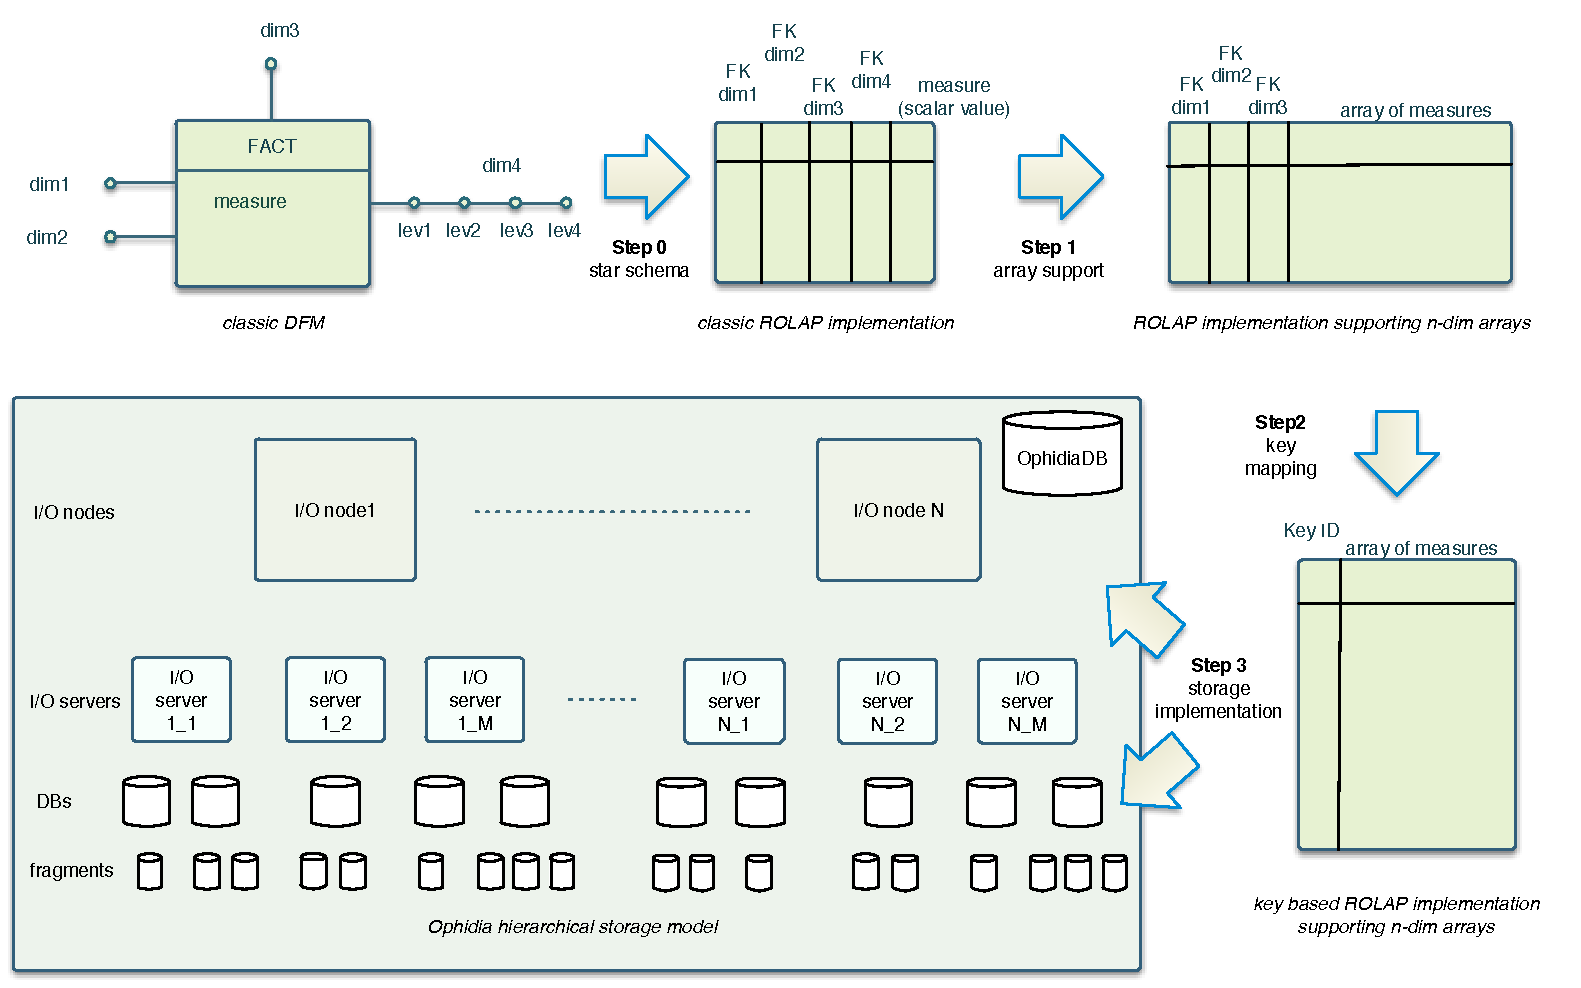
\includegraphics[width=\linewidth]{figures/Ophidia_storage_model.pdf}
	\caption{Moving from the DFM to the Ophidia hierarchical storage model}
	\label{fig: The Ophidia Storage Model}
\end{figure}

Let us consider the Dimensional Fact Model, a conceptual model for data warehouse and the classic Relational-OLAP (ROLAP) based implementation of the associated star schema. There is one fact table (FACT), four dimensions (dim1, dim2, dim3, and dim4), with the last dimension modelled through a 4-level concept hierarchy (lev1, lev2, lev3, lev4) and a single measure (measure). Let us consider a NetCDF output of a global model simulation where dim1, dim2, and dim3 correspond to latitude, longitude, and depth, respectively and dim4 is the time dimension, with the concept hierarchy year, quarter, month, day; measure represents, for instance, the air pressure.\\

\textbf{Ophidia internal storage model}\\

The Ophidia internal storage model is a two-step-based evolution of the star schema. Specifically, the first step includes the support for array-based data types while the second step includes a key mapping related to a set of foreign keys (fks). In this way, a multidimensional array can be managed using single tuple (e.g., an entire time series) and the n-tuple (fk\textunderscore dim1, fk\textunderscore dim2, ..., fk\textunderscore dimn) to be replaced by a single key (a numerical ID). It is worth noting that thanks to the second step the Ophidia storage model is independent of the number of dimensions, unlike the classic ROLAP-based implementation. Using this approach the system moves to a relational key-array schema supporting n-dimensional data management with a reduced disk space occupancy. The key attribute manages (through a single ID) a set of m dimensions (m<n), mapped onto the ID through a numerical function: \textit{ID = f(fk\textunderscore dim1, fk\textunderscore dim2, ..., fk\textunderscore dimm)}; the corresponding dimensions are called explicit dimensions. The array attribute manages the other n-m dimensions, called implicit dimensions.

In our example, latitude, longitude and depth are explicit dimensions, while time is the implicit one (in this case 1-D array) so the mapping on the Ophidia key-array data storage model consists of having a single table with two attributes:
\begin{itemize}
	\item an ID attribute: \textit{ID = f(fk\textunderscore latitudeID, fk\textunderscore longitudeID, fk\textunderscore depthID)} as a numerical datatype;
	\item an array-based attribute, managing the implicit dimension time, as a binary datatype.
\end{itemize}
In terms of implementation, several RDBMS allow data to be stored in binary form, but they do not provide a way to manage the array as a native datatype. The reason is that the available binary datatype does not look at the binary array as a vector, but rather as a single binary block: therefore, we have designed and implemented several array-based primitives to manage arrays stored through the Ophidia storage model.\\

\textbf{Hierarchical data management}\\

To manage large volumes of data, in the following, we discuss the horizontal partitioning technique that we use jointly with a hierarchical storage structure. Following the previous figure, it consists of splitting the central FACT table by ID into multiple smaller tables (each chunk is called \textit{fragment}). Many queries can execute more efficiently when using horizontal partitioning since it allows parallel query implementations and only a small fraction of the fragments may be involved in query execution (e.g., subsetting task). The fragments produced by the horizontal partitioning are mapped onto a hierarchical structure composed of four different levels:
\begin{itemize}
	\item Level 0: multiple I/O nodes (multi-host);
	\item Level 1: multiple instances of IO Server on the same I/O node (multi-IO Server);
	\item Level 2: multiple instances of databases on the same IO Server (multi-DB);
	\item Level 3: multiple fragments on the same database (multi-table).
\end{itemize}
The hierarchical data storage organisation allows data analysis and mining on a large set of distributed fragments as a whole exploiting multiple processes and parallel approaches.

\section{Big Data Concepts}

In the context of Big Data, there are many (often Java-based) technologies that address storing and processing of large quantities of data. \\

%\todo{each software solution as a paragraph?}
\textbf{Hadoop File System}\\
The Hadoop File System (HDFS) is a distributed file system that is designed to work with commodity hardware.
It provides fault tolerance via data replication and self-healing.
One limitation of its design is its consistency semantics which allows concurrent reads of multiple processes but only a single writer (WORM Model, write-once-read-many).
The data stored on HDFS are replicated in the cluster to ensure fault tolerance.
HDFS ensures data integrity and can detect loss of connectivity when a node is down.
The main concepts:

\begin{itemize}
	\item Datanode: nodes that own data;
	\item Namenode: a node that manages the file access operations.
\end{itemize}

The supported interfaces and languages are: HDFS Java API, WebHDFS REST API and libhdfs C API, as well as a Web interface and CLI shells.
Security is based on file authentication (user identity). However, HDFS accepts network protocols like Kerberos (for users) and encryption (for data).
HDFS was designed in Java for Hadoop Framework. Therefore any machine that supports Java can run it.
It can be considered as the ``source'' of many processing systems (especially in the Apache ecosystem) like Hadoop and Spark. All data stored into HDFS become ``sequence file'' files.

However, its sub-optimal performance on high-performance storage and assumption to work on cheap hardware makes it no optimal choice for HPC environments.
Therefore, many vendors support HDFS adapters on top of high-performance parallel file systems such as GPFS and Lustre.
One limitation of its design is its consistency semantics which allows concurrent reads of multiple processes but only a single writer.
\\

\textbf{HBase}\\
Apache HBase is a distributed, scalable, big data store.
HBase is an open-source, distributed, versioned, non-relational database modelled after Google's ``Bigtable: A Distributed Storage System for Structured Data'' by Chang et al. [R19]. Similarly to Bigtable, which leverages the distributed data storage provided by GFS, Apache HBase provides Bigtable-like capabilities on top of Hadoop and HDFS (https://hbase.apache.org/).
It can be used to perform random real-time read/write access to large volumes of data. HBase's goal is the hosting of large tables, on top of clusters of commodity hardware. As in the case of HDFS, this is not the optimal choice for HPC infrastructures. \\

\textbf{Hive}\\
Apache Hive is a data warehouse software facilitating reading, writing, and managing of large data sets residing in distributed storage using SQL (https://hive.apache.org/). It is built on top of Apache Hadoop and provides:
\begin{itemize}
	\item Tools to enable easy access to data via SQL, allowing data warehousing tasks such as ETL, reporting, and data analysis.
	\item Access to files stored directly in Apache HDFS or other data storage systems like Apache HBase.
The advantage is that no extract, transform or load (ETL) process is necessary. Just move the data into the file system and create a scheme on the existing files.
	\item support for query execution via various frameworks (i.e. Apache Tez, Apache Spark or MapReduce).
	\item A convenient SQL interface (including many of the later 2003 and 2011 features for analytics) to this data which allows users to explore data using SQL at a fine grain scale by accessing data stored on the file system.
\end{itemize}

\textbf{Drill}\\
Drill \footnote{\url{https://drill.apache.org}} also provides an SQL interface to existing data.

Similar to Hive, existing data can be adjusted, but in the case of Drill, data may be stored on various storage backends such as simple JSON file, on Amazon S3, or MongoDB.\\

\textbf{Alluxio}\\
Alluxio \footnote{\url{https://www.alluxio.com/docs/community/1.3/en/}} offers a scalable in-memory file system.
An interesting feature is that one can attach (mount) data from multiple (even remote) endpoints such as S3 into the hierarchical in-memory namespace.
It provides control to the in-memory data, for example, to trigger a flush of dirty data to the storage backend and an interface for pinning data in memory (similar to burst buffer functionality).
Data stored on Alluxio can be used on various big data tools.

%%%%%%%%%%%%%%%%%%%%%%%%%%%%%%%%%%%%%%%%%%%%%%%%%%%%%%%%%%%%%%%%%%%%%%%%%%%%%%%

\subsection{Ophidia Big Data Analytics Framework}
\label{sec: background/ophidia}

The Ophidia Big Data Analytics Framework falls in the big data analytics area applied to e-Science contexts.
%As introduced in \Cref{Ophidia Storage model}.
It addresses scientific use cases on large data volumes aiming at supporting the access, analysis and mining of n-dimensional array-based data. In this perspective, the Ophidia platform extends, in terms of both primitives and data types, current relational database systems enabling big data analytics tasks exploiting well-known scientific numerical libraries, a distributed and hierarchical storage model and a parallel software framework based on the Message Passing Interface to run from single operations to more complex dataflows. Further, Ophidia provides a server interface that makes the data analysis task a server-side activity in the scientific chain. Exploiting such an approach, most scientists would not need to download large volumes of data for their analysis as it happens today. On the contrary, they would download the results of their computations (typically in the megabytes or even kilobytes order) after running multiple remote data analysis operations.\\

In the following, the main features of the analytic framework of Ophidia will be depicted, the related architecture and the primitives and operators supported.\\

\textbf{The Ophidia architecture}\\

The Ophidia architecture consists of (i) the server front-end, (ii) the OphidiaDB, (iii) the compute nodes, (iv) the I/O nodes and (v) the storage system.
\begin{itemize}
	\item The server front-end is responsible for accepting and dispatching requests incoming from the clients. It is a pre-threaded server implementing standard interfaces (WS-I, OGC-WPS, GSI-VOMS). It relies on X.509 digital certificates for authentication and Access Control List (ACL) for authorisation;
	\item The OphidiaDB is the system (relational) database. By default the server front-end uses a MySQL database to store information about the system configuration and its status, available data sources, registered users, available I/O servers, and the data distribution and partitioning;
	\item The compute nodes are computational machines used by the Ophidia software to run the parallel data analysis operators;
	\item The I/O nodes are the machines devoted to the parallel I/O interface to the storage. Each I/O node hosts one or more I/O servers responsible for I/O with the underlying storage system. % described in \Cref{Ophidia Storage model}.
	\item The I/O servers are MySQL DBMSs or native in-memory services \cite{DBLP:conf/cd/EliaFDPFW16} supporting, at both the datatype and primitives levels, the management of n-dimensional array structures. This support has been adding a new set of functions (exploiting the User Defined Function approach, UDF) to manipulate arrays.
	\item The storage system is the hardware resource managing the data store, that is, the physical resources hosting the data according to the hierarchical storage structure. % defined in \Cref{Ophidia Storage model}.
\end{itemize}

\textbf{The Ophidia primitives and operators}\\

As mentioned before, the Ophidia framework addresses the analysis of n-dimensional arrays through a set of primitives included in the system as plugins (dynamic libraries). So far, about 100 primitives have been implemented. Multiple core functions of well-known numerical libraries (e.g. GSL, PETSc) have been included in new Ophidia primitives. Among others, the available array-based functions allow performing data sub-setting, data aggregation (i.e. max, min, avg), array concatenation, algebraic expressions, and predicate evaluation. It is important to note that multiple plugins can be nested to implement a single more complex array-based task.
Bit-oriented plugins have also been implemented to manage binary data cubes. Compression routines, based on zlib, xz, lzo libraries, are also available as array-based primitives.\\

Concerning the operators, The Ophidia analytics platform provides several MPI-based parallel functionalities to manipulate (as a whole) the entire set of fragments associated with a data cube. Some relevant examples include data cube sub-setting (slicing and dicing), data cube aggregation, array-based primitives at the data cube level, data cube duplication, data cube pivoting, and NetCDF file import and export.
Along with data operators, the framework provides a comprehensive set of metadata operators. Metadata represents a valuable source of information for data discovery and data description. From this point of view, some examples include provenance management, fragmentation and cube size information, variable and dimensions specific attributes.\\

\textbf{Workflows management}\\

The framework stack includes an internal workflow management system \cite{DBLP:conf/ieeehpcs/PalazzoMFDEWA15}, which coordinates and orchestrates the execution of multiple scientific data analytics and visualisation tasks (e.g. operational processing/analysis chains). It can manage the submission of complex scientific workflows using parsing and analysing input JSON files written in compliance with a predefined JSON Schema, which includes the description of each task, the definition of the dependencies among different tasks, and several metadata. In addition, advanced features as the definition of loops, variable definition and conditional statements are available. Workflow execution monitoring is allowed by explicitly querying the Ophidia server or in real-time through a graphical user interface.

\subsection{MongoDB}
The MongoDB\footnote{\url{https://docs.mongodb.com/}} is an open-source document database.
Its architecture is high-performant and horizontally scalable for cluster systems.
MongoDB offers a rich set of interfaces, e.g., RESTful access, C, Python, Java.

The data model of MongoDB provides three levels:
\begin{itemize}
  \item database: follows our typical notion; permissions are defined on the database level.
  \item Document: This is a BSON object (binary JSON) -- consisting of subdocuments with data.
  An example of JSON is shown in \Cref{lst:mongoJSON}.
  Each document has the primary key field: \_id. Either the field must be manually set, or it will be automatically filled.

  \item Collection: this is like a table of documents in a database. Documents can have individual schemas. It supports indices on fields (and compound fields).
\end{itemize}
To access data, one has to know the name of a database (potentially secured with a username and password), collection name. All documents within the collection can be searched or manipulated with one operation.

In the example of \Cref{lst:mongoJSON}, it would also be possible to create one document for each person and use the $\_id$ field with a self-defined unique ID such as a tax number.

\begin{tcbcode}[label={lst:mongoJSON}]{Example MongoDB JSON document}
\begin{lstlisting}
"_id" : ObjectId("43459bc2341bc14b1b41b124"),
"people" : [ # subdocuments:
    { "name" : "Max", "id" : 4711, "birth" : ISODate("2000-10-01")},
    { "name" : "Lena", "id" : 4712, "birth", ... }
  ]
\end{lstlisting}
\end{tcbcode}


MongoDB's architecture uses sharding of document keys to partition data across different servers.
Servers can be grouped into replica sets to provide high availability and fault tolerance.

\paragraph{Query documents}

A query document is a BSON document that is used to search all documents of a collection for data that matches the defined query.
The example in \Cref{lst:mongoQuery} specifies documents that contain the sub-documents people with an id field that is bigger than 4711.
Complex queries can be defined.
In combination with indices on fields, MongoDB can search large quantities of documents quickly.

\begin{tcbcode}[label={lst:mongoQuery}]{Example MongoDB Query document}
\begin{lstlisting}
{ "people.id" : { $gt : 4711 } }
\end{lstlisting}
\end{tcbcode}
